\documentclass{beamer}
\usepackage[T1]{fontenc}
\usepackage[utf8]{inputenc}
\usepackage[french]{babel}
\usepackage{geometry}
\usepackage{graphicx}
\usepackage{wrapfig}
\usepackage{indentfirst}
\usepackage{tikz}
\usepackage{igo}
\usepackage{amsfonts}
\usepackage{hyperref}

\graphicspath{{/home/pgi/TIPE/content/presentation/image/}}
\usetikzlibrary{trees}
\usetheme{Warsaw}
\expandafter\def\expandafter\insertshorttitle\expandafter{%
    \insertshorttitle\hfill%
    \insertframenumber\,/\,\inserttotalframenumber} 
% Title
\title{Morpion}
\author{Peng-Wei Chen, MP, \oldstylenums{2017}-\oldstylenums{2018}}
\date{}

\begin{document}
\tikzstyle{point}=[circle,draw,thin,fill=white]
\setbeamertemplate{navigation symbols}{}

%%fakesection title
\begin{frame}
    \titlepage
\end{frame}

%%fakesection introduction
\begin{frame}
    \frametitle{Introduction}
    \begin{itemize}
        \item La règle:\\
Deux joueurs jouent sur une grille de taille $15 \times 15$ sur le papier. Chacun prend un symbole et on dessine au tour par tour son symbole sur la grille. Le but est d'aligner 5 symboles verticalement, horizontalement ou en diagonale pour gagner.
        \pause
        \item (m, n, k)-jeu
        \pause
        \item La stratégie gagnante a été trouvée.
        
        \pause
        \item Les bornes inférieures.
    \end{itemize}
    
\end{frame}


%%fakesection Methode
\begin{frame}[t]
    \frametitle{Méthode}
    \begin{enumerate}
        \item On cherche tous les cas possibles.
            \begin{itemize}
                \item L'arbre de décision
% Figure: arbre de decision
                    \only<1>{
                        \gobansize{3}
                        \black{b2}
                        \copytogoban{2}
                        \white{a3}
                        \copytogoban{3}
                        \clear{a3}
                        \white{a2}
                        \copytogoban{4}
                        \cleargoban
                        \black{a2}
                        \copytogoban{5}
                        \clear{a2}
                        \black{a3}
                        \copytogoban{6}
                        \clear{a3}

                        \begin{tikzpicture}[level distance=1.5cm,
                            level 1/.style={sibling distance=2cm},
                        level 2/.style={sibling distance=1.3cm}]
                          \node {\showfullgoban}
                          child {node {\usegoban{2} \showfullgoban}
                              child {node {\usegoban{3} \showfullgoban}
                              child {node {$\vdots$}}}
                              child {node {\usegoban{4} \showfullgoban}
                              child {node {$\vdots$}}}
                            }
                            child {node {\usegoban{5} \showfullgoban}
                                child {node {$\vdots$}}
                                child {node {$\vdots$}}
                            }
                            child {node {\usegoban{6} \showfullgoban}
                                child {node {$\vdots$}}
                            child {node {$\vdots$}}
                        };
                        \end{tikzpicture}
                    }
                    \pause
                \item Complexité O(($m \times n$)!)
                    \pause
                \item{Fonction de valuation}
                    \pause
                \item k $\le$ 4
            \end{itemize}
        \item<6->On apparie les points de la grille. Si le deuxième joueur peut toujours prévenir la réussite du premier joueur en jouant le pairage, alors une telle stratégie n'existe pas.
            \begin{itemize}
                \item<7-> k > 7
            \end{itemize}

    \end{enumerate}
    \gobansize{10}
    \cleargoban
\end{frame}

%%fakesection fonction naive
\begin{frame}[t]
    \frametitle{Exploitation - k $\le$ 4}
    \framesubtitle{Fonction naïve}
    On considère le nombre de symboles non séparés dans une ligne.
    \begin{itemize}
        \item<2-> note d'un point sur la grille
        \item<3-> i-vivant / i-mort / mort
%% Exemple: 3-vivant, 3-mort
            \only<4>{
            \begin{center}
                \black{d5,e5,f5}
                \shortstack{\showgoban\\3-vivant\\$3^i$}
                \white{g5}
                \shortstack{\showgoban\\3-mort\\$3^{i-1}$}
            \\
            \ \\
                \white{c5}
                \clear{e5}
                \gobansymbol{e5}{A}
                \shortstack{\showgoban\\La note au point A est nulle pour le noir.}
                \cleargoban
            \end{center}
    En particulier, on donne $3^{k+1}$ au cas où le premier joueur est sûrement gagné, c'est-à-dire k-mort ou (k-1)-vivant. }
        \item<5-> L'effet de directions differentes
             
%% Exemple: 2 directions
            \only<6>{
            \begin{center}
                \black{d5,e5,f5,g3,g4,g6}
                \white{c5,g7}
                \black[\igotriangle]{g5}
                \gobansymbol{h5,g2}{x}
                \shortstack{\showgoban}
                \cleargoban
        \end{center}}
    \end{itemize}
\only<7>{La \og note \fg \ est la somme de ces valeurs selon les quatre directions.}
\end{frame}

%%fakesection exemple de note
\begin{frame}
    \frametitle{Exploitation - k $\le$ 4}
    \framesubtitle{Fonction naïve}
    \cleargoban

%% Exemple: note 
    \begin{center}
        \black{d5,e5,f5}
        \gobansymbol{g5}{A}
        \gobansymbol{e4}{B}
        \shortstack{\showfullgoban}
    \end{center}
    \center{La note au point \only<1>{A vaut 90 (81 + $3\times 3$).}\only<2>{B vaut 30 (3 + $3^2 \times 3$).}}
\end{frame}

%%fakesection minimax
\begin{frame}[t]
    \frametitle{Exploitation - k $\le$ 4}
    \framesubtitle{L'élagage alpha-beta}
%% Exemple: Besoin de alpha-beta
    On a besoin d'améliorer notre fonction.    
    \cleargoban
    \only<1>{
        \begin{center}
            \gobansize{5}
            \black[1]{c3}
            \white[2]{b4}
            \shortstack{\showfullgoban\\1}
            \cleargoban
            \black{c3}
            \white{b4}
            \white[\igotriangle]{b2,c2,d3,d4}
            \shortstack{\showfullgoban\\2}
            \cleargoban
            \black{c3,d3}
            \white{b4}
            \white[\igotriangle]{b3}
            \shortstack{\showfullgoban\\3}
        \end{center}}
        \begin{itemize}
            \item<2-> L'arbre de décision
            \item<3-> L'algorithme de minimax
        \end{itemize}

        \uncover<4->{
        Note = difference des notes de deux joueurs
%% Exemple: minimax
        \begin{center}
            \begin{tikzpicture}[level distance=1cm,
                level 1/.style={sibling distance=3cm},
                level 2/.style={sibling distance=3cm},
                level 3/.style={sibling distance=1cm}]
                \node[point] (n){\ }
                    child {node (n0){27}
                        child {node (n1){27}
                            child {node {4}}
                            child {node (n2){27}}
                            child {node {13}}
                        }
                        child {node (n3){29}
                            child {node {2}}
                            child {node {23}}
                            child {node (n4){29}}
                        }
                    }
                    child {node[point] (n5){\ }
                    child {node (n6){$\vdots$}}
                };
                \node[right of=n5,node distance=2cm] {max};
                \node[right of=n6,node distance=2cm] {min};
                \node[right of=n4,node distance=2.5cm] {max};
                \node[right of=n,node distance=3.5cm] {Origine};
                \only<5->{\draw[->,draw=red] (n2) -- (n1);}
                \only<6->{\draw[->,draw=red] (n4) -- (n3);}
                \only<7->{\draw[->,draw=red] (n1) -- (n0);}
                ;
            \end{tikzpicture}
        \end{center}
    }
%% Exemple?
    \uncover<8>{En pratique, on se donne une hauteur et on fait un parcours en profondeur.}
\end{frame}


%%fakesection alpha-beta
%alpha-beta
\begin{frame}
    \frametitle{Exploitation - k $\le$ 4}
    \framesubtitle{L'élagage alpha-beta}
    L'élagage alpha-beta
    \centering
    \begin{tikzpicture}
%%alpha
        \node[point] (n0){\ }
        child {node {81}}
        child {node[point] (n1){\ }
            child {node (n2){105}}
            child {node (n3){41}}
        }
        ;
        \node[right of=n1,node distance=2cm] {max};
        \node[right of=n3,node distance=1.3cm] {min};
        \node[below of=n2,node distance=0.5cm] {Coupure alpha};
        \draw[-] (n3) to node{X} (n1);
        \draw[-] (n1) to node{X} (n0);
%%beta
        \node[point,right of=n0,node distance=7cm] (n){\ }
        child {node {40}}
        child {node[point] (n4){\ }
            child {node (n5){35}}
            child {node (n6){77}}
        }
        ;
        \node[right of=n4,node distance=2cm] {min};
        \node[right of=n6,node distance=1.3cm] {max};
        \node[below of=n5,node distance=0.5cm] {Coupure beta};
        \draw[-] (n6) to node{X} (n4);
        \draw[-] (n4) to node{X} (n);
    \end{tikzpicture}
    coupure alpha: niveau max\\
    coupure beta: niveau min
\end{frame}



%%fakesection intro de k>=8
%% k >= 8
\begin{frame}
    \frametitle{Exploitation - k $\ge$ 8}
    Le premier joueur n'a pas de stratégie gagnante lorsque k~=~8.
%% m-n-9
\end{frame}

%%fakesection m-n-9
\begin{frame}
    \frametitle{Exploitation - k $\ge$ 8}
    \framesubtitle{Preuve du cas k~=~9}
    \only<1>{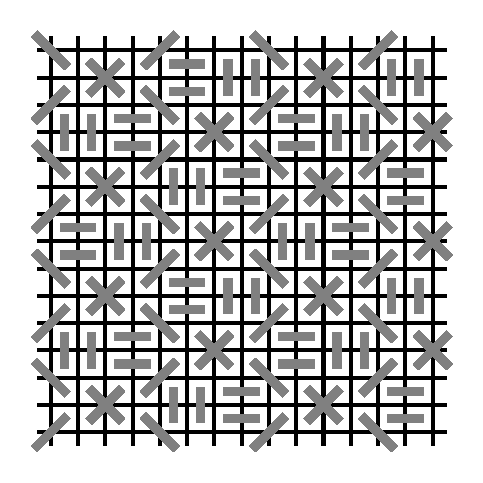
\includegraphics{m-n-9-clear.eps}}
    \only<2>{\includegraphics{m-n-9-horizon.eps}}
    \only<3>{\includegraphics{m-n-9-vertical.eps}}

\end{frame}

%%fakesection sous-jeu
\begin{frame}
    \frametitle{Exploitation - k $\ge$ 8}
    \framesubtitle{Preuve du cas k~=~8}
%% sous-jeu
    Sous-jeu\\
    \centering
    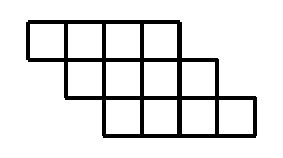
\includegraphics{m-n-8-little.eps}
\end{frame}

%%fakesection regle de sous-jeu
\begin{frame}
    \frametitle{Exploitation - k $\ge$ 8}
    \framesubtitle{Preuve du cas k~=~8}
    Règle du sous-jeu: trois façons pour gagner.
    \begin{itemize}
        \uncover<2->{\item Aligner trois symboles en diagonale.}
        \uncover<3->{\item Aligner verticalement deux symboles.}
        \uncover<4->{\item Aligner horizontalement quatre symboles.}
%% regle de sous-jeu
        \begin{center}
            \uncover<2->{\includegraphics[height=1.5cm]{8-rules1.eps}}
            \uncover<3->{\includegraphics[height=1.5cm]{8-rules2.eps}}
            \uncover<4->{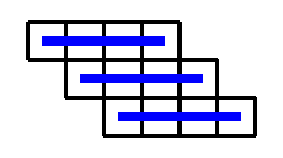
\includegraphics[height=1.5cm]{8-rules3.eps}}
        \end{center}
\end{itemize}
\end{frame}

%%fakesection m-n-8
\begin{frame}
    \frametitle{Exploitation - k $\ge$ 8}
    \framesubtitle{Preuve du cas k~=~8}
    On divise la grille initialle en des grilles du sous-jeu. 
%% m-n-8
    \only<1>{\includegraphics[height=5cm]{8-sol-initial.eps}}
    \only<2>{\includegraphics[height=5cm]{8-sol-straight.eps}}
    \only<3>{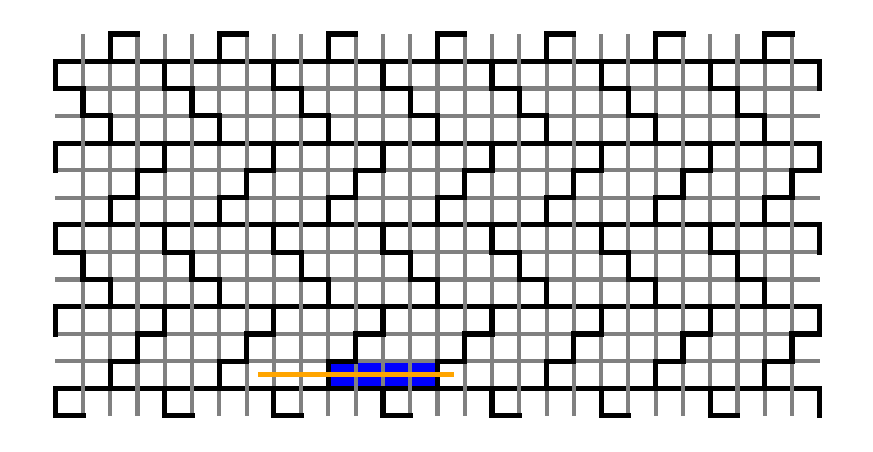
\includegraphics[height=5cm]{8-sol-horizontal.eps}}
    \only<4>{\includegraphics[height=5cm]{8-sol-diagonal.eps}}
    \only<5>{\includegraphics[height=5cm]{8-sol.eps}}
    
\end{frame}

%%fakesection conclusion
\begin{frame}
    \frametitle{Conclusion}
On suppose que $m \le n$.\\
\uncover<2->{Dans le cas où $k \le 4$, une telle stratégie existe lorsque}
\begin{itemize}
    \item<3-> k = 3\\
        $m \ge 3$, $n \ge 4$
    \item<4-> k = 4\\
        $m \ge 4$, $n \ge 5$
\end{itemize}
\uncover<5->{Dans le cas où $k \ge 8$, il n'existe pas une stratégie gagnante pour le premier joueur.}
\end{frame}

\end{document}
